\documentclass[graphics]{beamer}

\usepackage{graphicx}
\usepackage{verbatim}
\usepackage{wrapfig}
\useoutertheme{shadow}
%\usecolortheme{orchid}
\usecolortheme{seahorse}


% math commands
\newcommand{\be}{\begin{eqnarray}}
\newcommand{\ee}{\end{eqnarray}}
\newcommand{\beq}{\begin{equation}}
\newcommand{\eeq}{\end{equation}}
\def\simless{\mathbin{\lower 3pt\hbox
      {$\rlap{\raise 5pt\hbox{$\char'074$}}\mathchar"7218$}}}
\def\simgreat{\mathbin{\lower 3pt\hbox
      {$\rlap{\raise 5pt\hbox{$\char'076$}}\mathchar"7218$}}} %> or of order

% variables

\def\toonscale{0.45}
\def\mboxy#1{\mbox{\small #1}}


\begin{comment}
\AtBeginSection[]{
  \frame{
    \frametitle{Outline}
    \tableofcontents[currentsection]
  }
}
\end{comment}

%\title{Probing Space and Time}
%\subtitle{}
\author[U. Pen]{Ue-Li Pen
\\%[8mm] 
image credit: Andre Recnik}
}
\date{March 11, 2016}


\begin{document}

\frame{
\begin{picture}(320,250)
\put(-50,20){
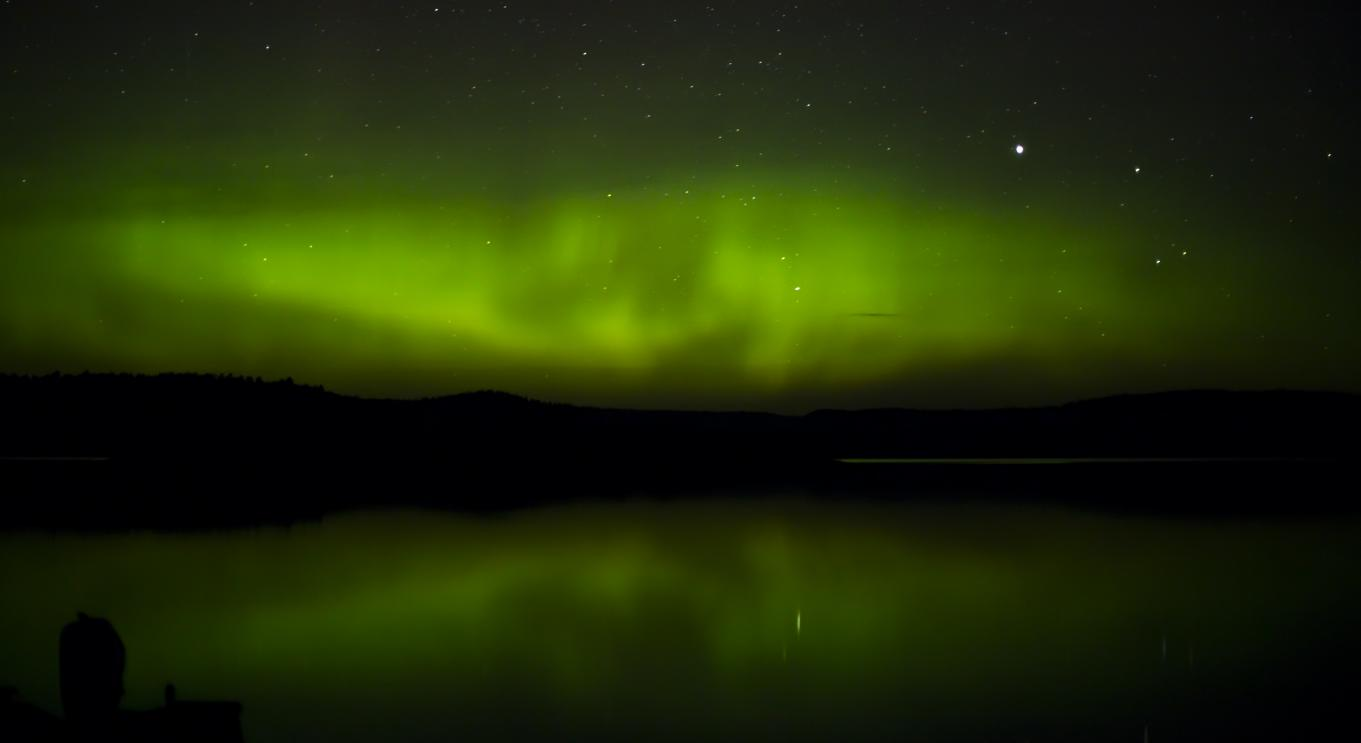
\includegraphics[width=5.5in]{Figures/traverse-aurora.jpg}}
%\textcolor{red}{
\end{picture}
%\vspace{-0.2in}image credit: Andre Recnik\vspace{-0.3in}
%\vspace{-2.5in}
%\titlepage
}

%\section*{Introduction}
\section{probing space-time}

\begin{comment}
  \subsection{Outline}

  \frame{
    \frametitle{Outline}
    \tableofcontents
  }
\end{comment}

  \frame{
\vspace{-0.5in}
    \frametitle{Gravitational Waves}
    \begin{itemize}
        \item ripples in space-time
        \item recently detected in LIGO
        \item potentially detectable by pulsars, CMB, 21cm
        \item new cosmological sources (1510.02985,1601.03917)
        \item new tools to measure and classify
    \end{itemize}
  }
  \frame{
    \frametitle{Scintillometry}
    \begin{itemize}
        \item use interstellar plasma as telescope
        \item unprecedented angular precision: 50 picoarcseconds
        \item test GR, measure neutron star mass, localize
          gravitational wave sources
    \end{itemize}
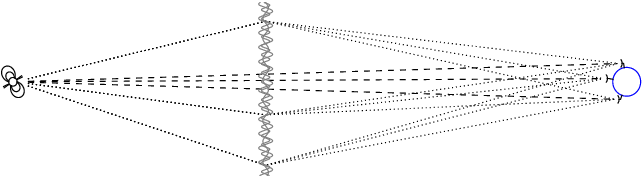
\includegraphics[width=4.5in]{Figures/scintillometry.png}
}

\end{document}
